% CVPR 2022 Paper Template
% based on the CVPR template provided by Ming-Ming Cheng (https://github.com/MCG-NKU/CVPR_Template)
% modified and extended by Stefan Roth (stefan.roth@NOSPAMtu-darmstadt.de)

\documentclass[10pt,twocolumn,letterpaper]{article}

%%%%%%%%% PAPER TYPE  - PLEASE UPDATE FOR FINAL VERSION
\usepackage[review]{cvpr}      % To produce the REVIEW version
%\usepackage{cvpr}              % To produce the CAMERA-READY version
%\usepackage[pagenumbers]{cvpr} % To force page numbers, e.g. for an arXiv version

% Include other packages here, before hyperref.
\usepackage{graphicx}
\usepackage{amsmath}
\usepackage{amssymb}
\usepackage{booktabs}


% It is strongly recommended to use hyperref, especially for the review version.
% hyperref with option pagebackref eases the reviewers' job.
% Please disable hyperref *only* if you encounter grave issues, e.g. with the
% file validation for the camera-ready version.
%
% If you comment hyperref and then uncomment it, you should delete
% ReviewTempalte.aux before re-running LaTeX.
% (Or just hit 'q' on the first LaTeX run, let it finish, and you
%  should be clear).
\usepackage[pagebackref,breaklinks,colorlinks]{hyperref}


% Support for easy cross-referencing
\usepackage[capitalize]{cleveref}
\crefname{section}{Sec.}{Secs.}
\Crefname{section}{Section}{Sections}
\Crefname{table}{Table}{Tables}
\crefname{table}{Tab.}{Tabs.}


%%%%%%%%% PAPER ID  - PLEASE UPDATE
\def\cvprPaperID{*****} % *** Enter the CVPR Paper ID here
\def\confName{CVPR}
\def\confYear{2022}


\begin{document}

%%%%%%%%% TITLE - PLEASE UPDATE
\title{
Positional Information Causally Constrains Background Shortcut Reliance in Vision Transformer Models
}

\author{First Author\\
Institution1\\
Institution1 address\\
{\tt\small firstauthor@i1.org}
% For a paper whose authors are all at the same institution,
% omit the following lines up until the closing ``}''.
% Additional authors and addresses can be added with ``\and'',
% just like the second author.
% To save space, use either the email address or home page, not both
\and
Second Author\\
Institution2\\
First line of institution2 address\\
{\tt\small secondauthor@i2.org}
}
\maketitle

%%%%%%%%% ABSTRACT
\begin{abstract}
   Vision Transformers (ViTs) match or exceed the strongest architectures for object recognition, but, like Convolutional Neural Networks (CNNs), they can exploit image backgrounds rather than focused objects. Whether a ViT's positional encoding causally governs this reliance has not been thoroughly tested in literature, and it is commonly assumed that newer rotary encodings (RoPE) resist such shortcuts better than absolute encodings (APE). In this work, we probe this assumption by scaling the positional signal of eight identically trained ViT checkpoints and measuring their resulting changes in background reliance on ImageNet-9. We find that attenuating the positional signal monotonically raises background reliance in every model (e.g.\ $5.1 \rightarrow 12.8$ pp), that the encoding scheme is irrelevant, and that the effect is specific to spatial information loss, not generic degradation. These findings extend to the Waterbirds dataset~\cite{sagawa2020}. We investigate several mechanisms and find little evidence any single mechanism carries the effect.
\end{abstract}

%%%%%%%%% BODY TEXT
%------------------------------------------------------------------------
\section{Introduction}
\label{sec:intro}

\subsection{The Robustness Problem}
Robust object recognition requires a model to make its decisions principally on the foreground object, not its surroundings. Modern recognition models, including Vision Transformers (ViTs), are known to exploit background shortcuts; for instance, by predicting a class of image as a ``fish'' from surrounding water rather than from the fish itself~\cite{xiao2021,geirhos2020}. Such reliance is invisible on standard tests but causes failures when the backgrounds are not correlated to the training, for instance, by virtue of a new environment~\cite{sagawa2020}. Understanding what keeps a model's attention spatially on the object is therefore central to its robustness.

\subsection{The Overlooked Lever and Precedence to Overturn}
A ViT processes an image as an unordered set of patches, depending on positional information to recover the spatial layout. Two schemes remain the most prevalent: absolute positional encodings (APE), which add learned per-position offsets, and rotary encodings (RoPE), which form positions as phase rotations~\cite{heo2024}. Because RoPE encodes relative geometry, it is widely assumed to support more robust spatial reasoning, thus being better at resisting background shortcuts than APE. This intuition, however, has not been clearly tested in the literature against background reliance. More fundamentally, it is unknown whether the positional signal causally governs the shortcut at all.

\subsection{Research Question \& Approach}
Our contributions are:
\begin{itemize}
    \item We show, causally, that attenuating the functional positional signal monotonically increases background reliance across all eight checkpoints (e.g., $5.1 \rightarrow 12.8$ pp), isolated by a within-model dissociation between functional and vestigial signals.
    \item We establish that this effect is encoding agnostic: APE and RoPE are statistically equivalent, with a powered null $\le 2$ pp, overturning the common assumption that rotary encodings resist the shortcut better.
    \item We show the effect is specific to spatial-informational loss rather than generic degradation, the effect generalizes to a second spurious benchmark (Waterbirds)~\cite{sagawa2020}, and, through investigations of several candidate mechanisms, the effect resists single-channel localization.
\end{itemize}

\Cref{fig:method} summarizes our setup and the main result.

%------------------------------------------------------------------------
\section{Related Work}

\noindent\textbf{Background bias and spurious correlations.} Prior work establishes that object-recognition models often exploit background elements or other non-causal factors. Contextual bias research precedes deep learning~\cite{torralba2003,zhang2007}, and Geirhos et al.~\cite{geirhos2020} later framed it as shortcut learning. Xiao et al.~\cite{xiao2021} made the effect measurable by constructing ImageNet-9 / the Backgrounds Challenge, quantifying the reliance differences between backgrounds and foregrounds. This paper is also the source of the BG-Gap metric we adopt. Waterbirds~\cite{sagawa2020} provides a spurious cue, and methods such as DFR~\cite{kirichenko2023} and background masking~\cite{aniraj2023} decrease the bias. These works characterize or remove the shortcut rather than uncovering what internal signals characterize or causally decrease it. With regards to our work, we build upon these findings that characterize or remove background shortcuts by searching for their causative internal factors.

\noindent\textbf{Positional encodings in Vision Transformers.} Because self-attention is permutation-invariant, ViTs require an explicit positional signal~\cite{dosovitskiy2021}. Absolute positional encodings (APE) add learned per-position offsets while relative and rotary encodings store geometry between tokens. Wu et al.~\cite{wu2021} systematized relative encodings for vision, and Heo et al.~\cite{heo2024} introduced 2D rotary encodings (RoPE-Axial, RoPE-Mixed). Touvron et al.~\cite{touvron2022} provides the DeiT-III checkpoints we use.

\noindent\textbf{Causal and mechanistic analysis.} Within ViTs, interpretability studies have identified register / artifact tokens (high-norm tokens that process global information rather than patch-level findings)~\cite{darcet2024} and cautioned that raw attention is a poor explanatory factor~\cite{jain2019}. We act as interventionists, manipulating a single signal on frozen weights, but apply it to the positional signal and to a behavioral shortcut metric, and we report negative mechanism findings.

\begin{figure*}[t]
  \centering
  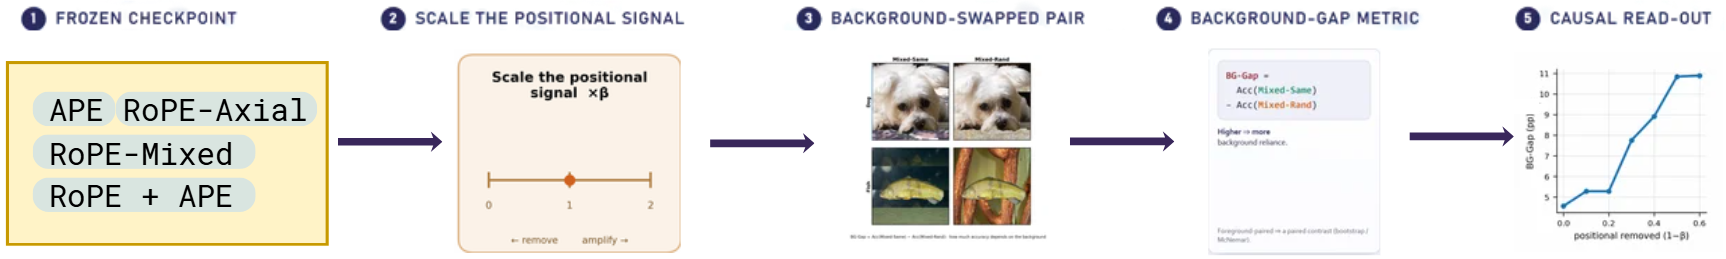
\includegraphics[width=\linewidth]{figures/pipeline.png}
  \caption{\textbf{Within-checkpoint positional intervention (no retraining).}
    A frozen, identically-trained ViT is evaluated on a background-swapped pair
    (\textsc{Mixed-Same}/\textsc{Mixed-Rand}); only the positional signal is scaled by
    $\beta$, and we read off $\mathrm{BG\text{-}Gap}=\mathrm{Acc}(\textsc{Mixed-Same})-
    \mathrm{Acc}(\textsc{Mixed-Rand})$. Because the weights are never updated, any change
    in $\mathrm{BG\text{-}Gap}$ is caused by the positional signal.}
  \label{fig:method}
\end{figure*}

%------------------------------------------------------------------------
\section{Methodology}

Broadly, we aim to test whether positional signal, when isolated, controls background-shortcut reliance. We describe the models (\cref{sec:models}), the benchmark and metric (\cref{sec:metric}), the intervention (\cref{sec:intervention}) and its control (\cref{sec:funcvest}), the accuracy-matched specificity controls (\cref{sec:specificity}), the interpretability guard (\cref{sec:guard}), our statistical approach (\cref{sec:stats}), the cross-dataset generality test (\cref{sec:waterbirds}), and the mechanism probes (\cref{sec:probes}). \Cref{fig:method} summarizes the general pipeline.

\subsection{Models}
\label{sec:models}
We study eight DeiT-III Vision Transformers from the public RoPE-ViT release~\cite{heo2024,touvron2022}. These models are identical in architecture, training data, and recipe, differing only in their positional encoding. Their positional encodings are APE, RoPE-Axial, RoPE-Axial + APE, RoPE-Mixed, and RoPE-Mixed + APE with five ViT-S/16 and three ViT-B/16. RoPE-Axial applies rotary embeddings independently along vertical and horizontal axes. RoPE-Axial + APE combines axial rotary encoding with absolute positional encoding to allow models to both have relative and absolute spatial information. RoPE-Mixed uses a learned mixture of horizontal and vertical components to provide a more flexible representation than RoPE-Axial. RoPE-Mixed + APE augments mixed rotary positional encoding with absolute positional encoding, allowing for the most flexible representation. We use the released checkpoints and train no models, removing training factors as confounds. Importantly, this introduces the limitation (\cref{sec:limitations}) of a single seed per encoding. All models are loaded by explicit checkpoint restoration. \Cref{tab:models} lists the models and their clean ImageNet-9 accuracies.

\begin{table}[t]
  \centering\small
  \begin{tabular}{@{}lcc@{}}
    \toprule
    Encoding & Scales & Clean Acc.\ (\%) \\
    \midrule
    APE              & S, B & 97.1 \\
    RoPE-Axial       & S    & 97.3 \\
    RoPE-Axial + APE & S    & 97.1 \\
    RoPE-Mixed       & S, B & 97.2 \\
    RoPE-Mixed + APE & S, B & 97.4 \\
    \bottomrule
  \end{tabular}
  \caption{The eight matched checkpoints (five ViT-S/16, three ViT-B/16), differing only in positional encoding. Accuracy is clean ImageNet-9 top-1 for the ViT-S/16 models; the three ViT-B/16 models score $\sim$98\%.}
  \label{tab:models}
\end{table}

\subsection{Benchmark \& Metrics}
\label{sec:metric}
We measure background reliance on ImageNet-9 / the Backgrounds Challenge~\cite{xiao2021}, a nine-class benchmark with foreground-paired variants---a fixed foreground object composed onto different backgrounds, separated by class. We use two main variants: \textsc{Mixed-Same} places the object on a randomly chosen same-class background and \textsc{Mixed-Rand} on a random-class background. We quantify reliance as the background gap,
%
\begin{equation}
  \mathrm{BG\text{-}Gap} \;=\; \mathrm{Acc}(\textsc{Mixed-Same}) - \mathrm{Acc}(\textsc{Mixed-Rand}),
  \label{eq:bggap}
\end{equation}
%
where larger values indicate greater dependence on the background. Because each foreground appears in both variants, \cref{eq:bggap} is a \emph{paired} contrast, which enables the paired statistics of \cref{sec:stats}. Predictions from the 1000-way ImageNet head are mapped into the nine main classes.

\subsection{The Causal Intervention}
\label{sec:intervention}
We use a within-checkpoint intervention on the \emph{frozen} positional parameters. For a model and scale factor $\beta$, we (i)~snapshot the positional parameters, (ii)~replace them with a $\beta$-scaled copy, (iii)~run inference over all variants, and (iv)~restore the original parameters. For APE, we scale the additive positional embedding $\mathbf{P}$, and for RoPE we scale the rotation angle $\theta_p$ applied to queries and keys at position $p$:
%
\begin{equation}
  \mathbf{P}(\beta)=\beta\,\mathbf{P}\quad(\text{APE}),
  \qquad
  \theta_p(\beta)=\beta\,\theta_p\quad(\text{RoPE}).
  \label{eq:intervention}
\end{equation}
%
Thus $\beta{=}1$ does not modify the model, $\beta{=}0$ removes all positional information, and $\beta{>}1$ amplifies positional information; we sweep $\beta\in[0,1]$ for attenuation (and $[1,2]$ for amplification) in steps of $0.1$. Importantly, the weights are never updated and only $\beta$ changes between runs, so any changes in $\mathrm{BG\text{-}Gap}$ are attributable to effects stemming from positional signal. \Cref{fig:method} depicts the general pipeline. We verify the effect is not an artifact resulting from this particular scaling by reproducing it with two alternative attenuations: spatial low-pass of $\mathbf{P}$ and rotary-frequency truncation.

\subsection{Functional vs.\ Vestigial Signal}
\label{sec:funcvest}
Hybrid models carry both an APE and a RoPE signal but use only one. We define the \emph{functional} signal as the one the architecture relies on and the \emph{vestigial} signal as the unused remainder. Importantly, the unused remainder remains present in the forward computation and can, in principle, influence predictions. We apply the intervention of \cref{sec:intervention} to each separately. This yields a control---if it is the used positional information that constrains the shortcut, only the functional knob should move $\mathrm{BG\text{-}Gap}$. Because the contrast is internal to a single frozen checkpoint, it is not affected by the single-seed limitation of lacking cross-encoding comparisons.

\subsection{Accuracy-Matched Specificity Controls}
\label{sec:specificity}
To establish that the effect is specific to spatial information rather than destructive interference on the model, we compare positional attenuation against four non-positional corruptions, each swept to the same accuracy as the positional intervention. Patch-wise noise and channel dropout are used to decrease feature fidelity without removing spatial layout. Two spatial controls remove spatial evidence by other means (token dropout, attention-temperature flattening). For each control we report the excess $\mathrm{BG\text{-}Gap}$ of positional attenuation at matched accuracy. This is obtained by interpolating each curve to a common accuracy and differencing. A positive excess over a control indicates the positional effect is not explained by that control's failure mode, thereby isolating the spatial information-relevant variables.

\subsection{Interpretability Guard}
\label{sec:guard}
We note that $\mathrm{BG\text{-}Gap}$ is interpretable only while the model maintains a certain baseline of performance. Once an intervention collapses towards chance, the gap becomes non-monotonous and no longer measures background reliance. We therefore impose a floor and interpret $\mathrm{BG\text{-}Gap}$ only where \textsc{Original}-image accuracy exceeds $0.80$ on ImageNet-9 ($0.70$ on Waterbirds, \cref{sec:waterbirds}). Points beyond the floor are shown for completeness with open markers but are excluded from slopes and tests. $0.8$ and $0.7$ were empirically chosen as conservative lower bounds based on non-attenuated model performance on their respective datasets.

\subsection{Statistics}
\label{sec:stats}
All evaluations are logged per image, allowing for paired inference over the foreground-paired structure. We report 95\% confidence intervals from a paired bootstrap that resamples foreground identities (the clustering unit), McNemar tests for paired accuracy differences, and, to compare the encodings, two one-sided tests (TOST) of equivalence at a $2$\,pp margin. Monotone dose-response is summarized by Spearman $\rho$ with a bootstrap slope CI. Cross-encoding multiplicity is controlled by Benjamini--Hochberg FDR across the eight models. A power analysis run across the models gives a minimum detectable effect of $1.6$\,pp at $80\%$ power, which justifies our equivalence result as a powered null rather than a lack of evidence.

\subsection{Generality Protocol: Waterbirds}
\label{sec:waterbirds}
To test generality on a mechanistically different spurious cue, we repeat the process on Waterbirds~\cite{sagawa2020}, where bird species are spuriously correlated with land and water backgrounds. We train a single linear ERM head on frozen ViT-S features under the natural $95\%$-spurious distribution---so the head \emph{learns} the shortcut. Importantly, we hold it fixed across the $\beta$ sweep, as refitting per every value of $\beta$ would erase the effect we intend to study. We measure the spurious gap $\mathrm{Acc}(\text{congruent})-\mathrm{Acc}(\text{incongruent})$, reporting its accuracy-guarded change under positional removal.

\subsection{Candidate-Mechanism Probes}
\label{sec:probes}
Finally, we empirically probe four candidate mechanisms for the effect. We test whether (i)~high-norm register tokens~\cite{darcet2024} in background patches predict per-image reliance, (ii)~a causal attention-temperature sweep can reproduce the positional effect, (iii)~a linear probe can recover the background class from frozen features as the position is attenuated, and (iv)~a specific high-frequency rotary band shows the effect at a matched accuracy. While results proved middling, they appear in \cref{sec:mechanisms}.

%------------------------------------------------------------------------
\section{Experiments and Results}
\label{sec:results}

\subsection{Position Causally Constrains the Shortcut}
We first test if attenuating the positional signal raises background reliance in the ViT checkpoints. Sweeping $\beta$ from $1$ to $0$ on each frozen model (\cref{fig:dose}, left), $\mathrm{BG\text{-}Gap}$ increases monotonically in all 8/8 checkpoints, with Spearman $\rho \ge 0.98$ and bootstrap slope CIs excluding zero. All of these results pass BH-FDR at $p \approx 0$. The effect holds at both model scales and for all encoding family permutations. Degrading the vestigial signal in hybrids does nothing (\cref{fig:dose}, right): its slope brackets zero, and the functional-minus-vestigial difference excludes zero, isolating the effect to the positional information the model uses. Amplifying position ($\beta > 1$) does not lower $\mathrm{BG\text{-}Gap}$, as every CI crosses zero.

\begin{figure*}[t]
  \centering
  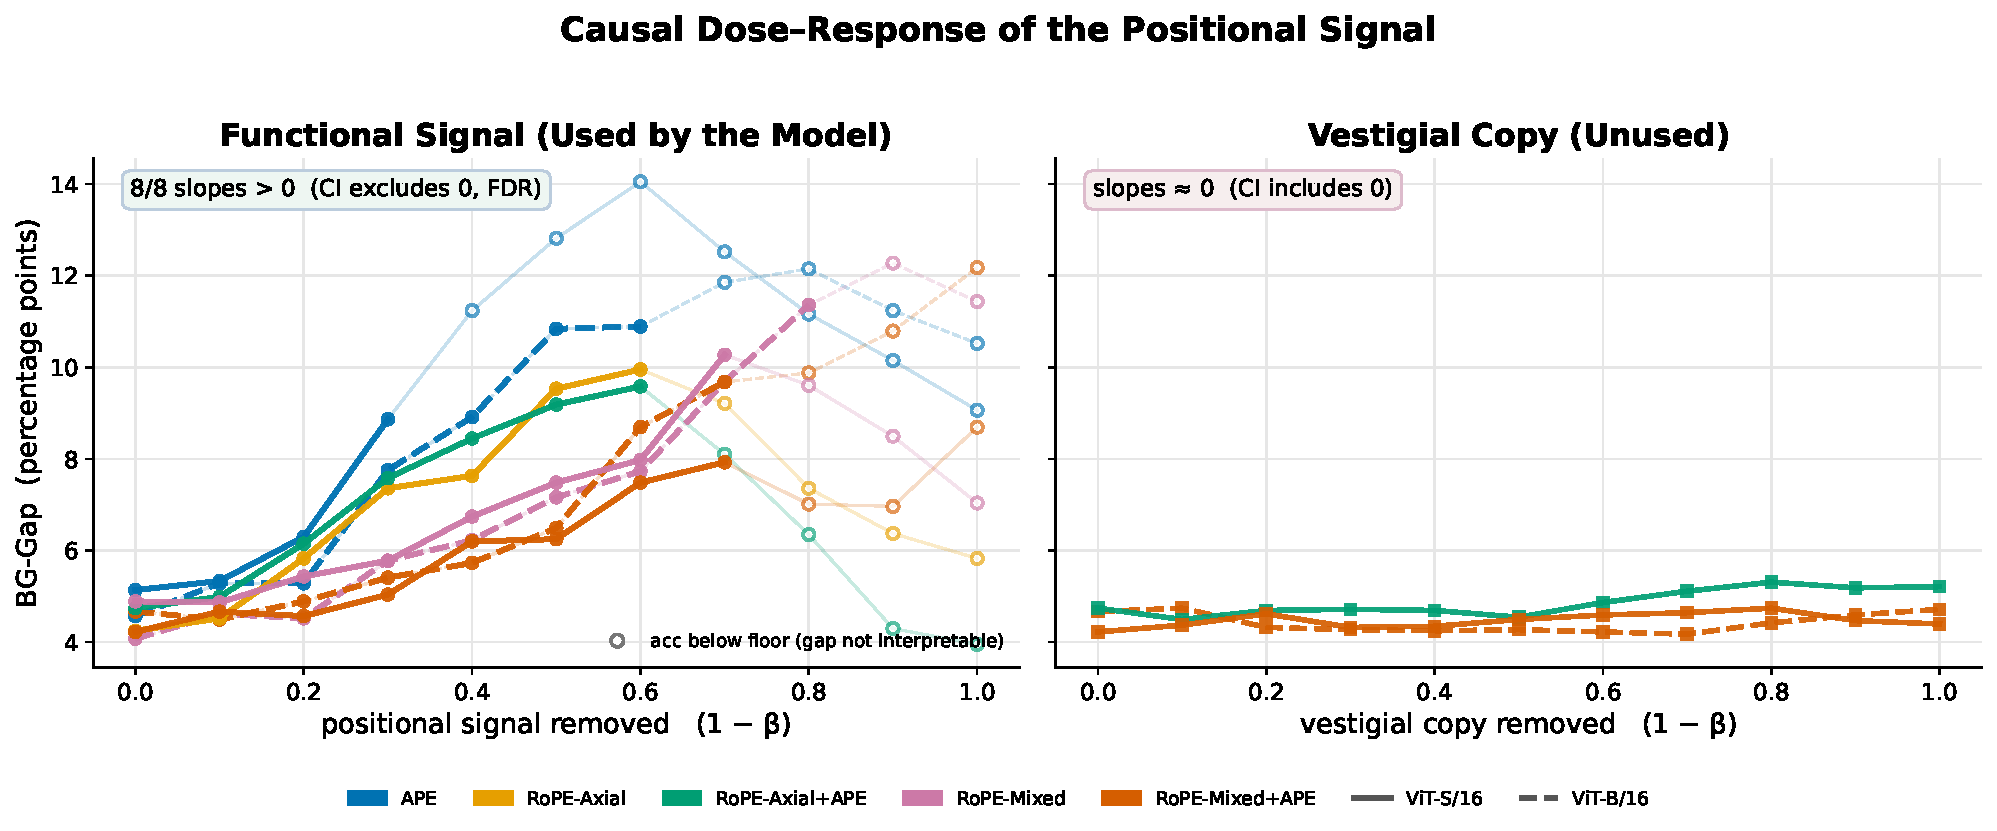
\includegraphics[width=\linewidth]{figures/03_dose_response.pdf}
  \caption{\textbf{Attenuating the functional positional signal causally raises background reliance
    (8/8), while the vestigial signal is inert.} $\mathrm{BG\text{-}Gap}$ vs.\ positional removal
    $(1-\beta)$; solid = above the interpretability floor, open = below. \emph{Left:} functional signal.
    \emph{Right:} vestigial copy.}
  \label{fig:dose}
\end{figure*}

\subsection{The Effect Is Encoding-Agnostic}
We test if the encoding scheme changes results. Across the five encodings, intact $\mathrm{BG\text{-}Gap}$ spans only $4.2$--$5.1$\,pp (\cref{fig:forest}); under a paired test no pair differs (largest, APE$-$Axial, $+0.94$\,pp, CI $[-0.22,+2.10]$), and every pair is TOST-equivalent at a $2$\,pp margin ($6/10$ at $1.5$\,pp). With a minimum detectable effect of $1.6$\,pp, this is a demonstrated equivalence between the encoders, not a failure to reject findings. APE and RoPE are shown concentrating positional energy in the same low-frequency band through a 2D-Fourier analysis, helping explain why the models are interchangeable.

\begin{figure}[t]
  \centering
  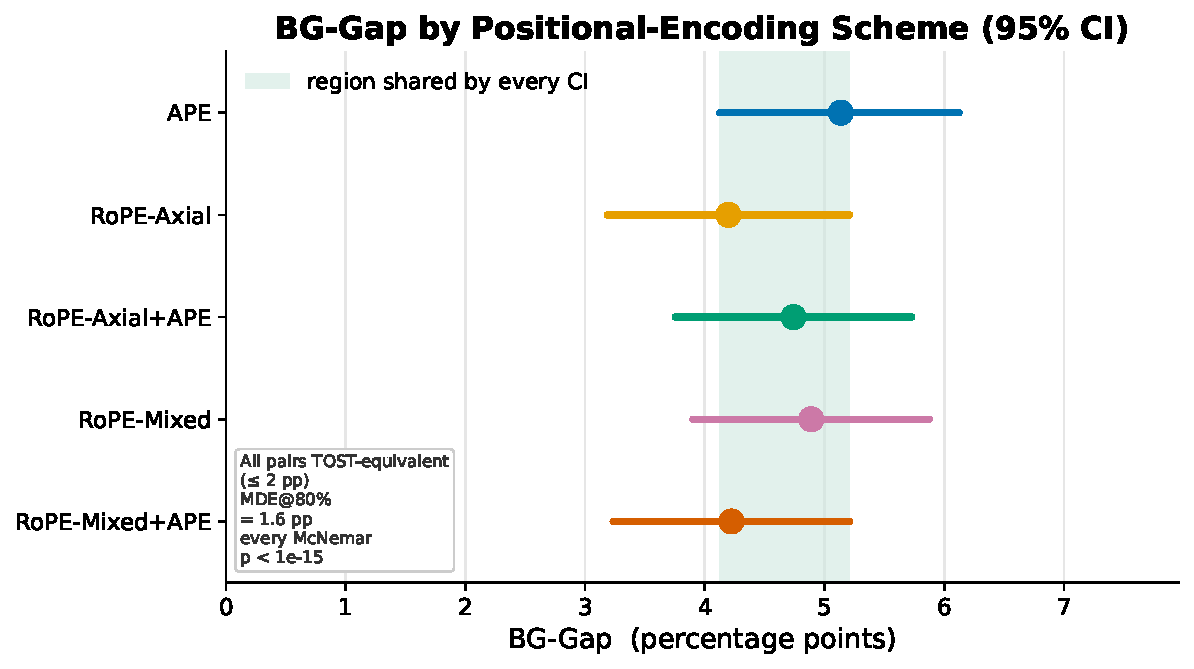
\includegraphics[width=\linewidth]{figures/02_forest_powered_null.pdf}
  \caption{\textbf{The encoding scheme is irrelevant.} Intact $\mathrm{BG\text{-}Gap}$ by encoding with
    95\% CIs; all pairs are TOST-equivalent at $\le\!2$\,pp (MDE $1.6$\,pp): a powered null.}
  \label{fig:forest}
\end{figure}

\subsection{The Effect Is Specific to Spatial Information}
We test if any accuracy-matched degradation would have a similar effect. Matching each control to the positional intervention's clean accuracy (\cref{fig:specificity}), positional attenuation induces $+3.8$\,pp excess $\mathrm{BG\text{-}Gap}$ over patch-noise and $+1.3$\,pp over attention-temperature, with CIs excluding zero (\cref{tab:specificity}). The two spatial controls are comparable, seemingly serving as evidence against the thesis. Their comparability, however, because they too remove spatial information, reinforces the thesis.

\begin{figure}[t]
  \centering
  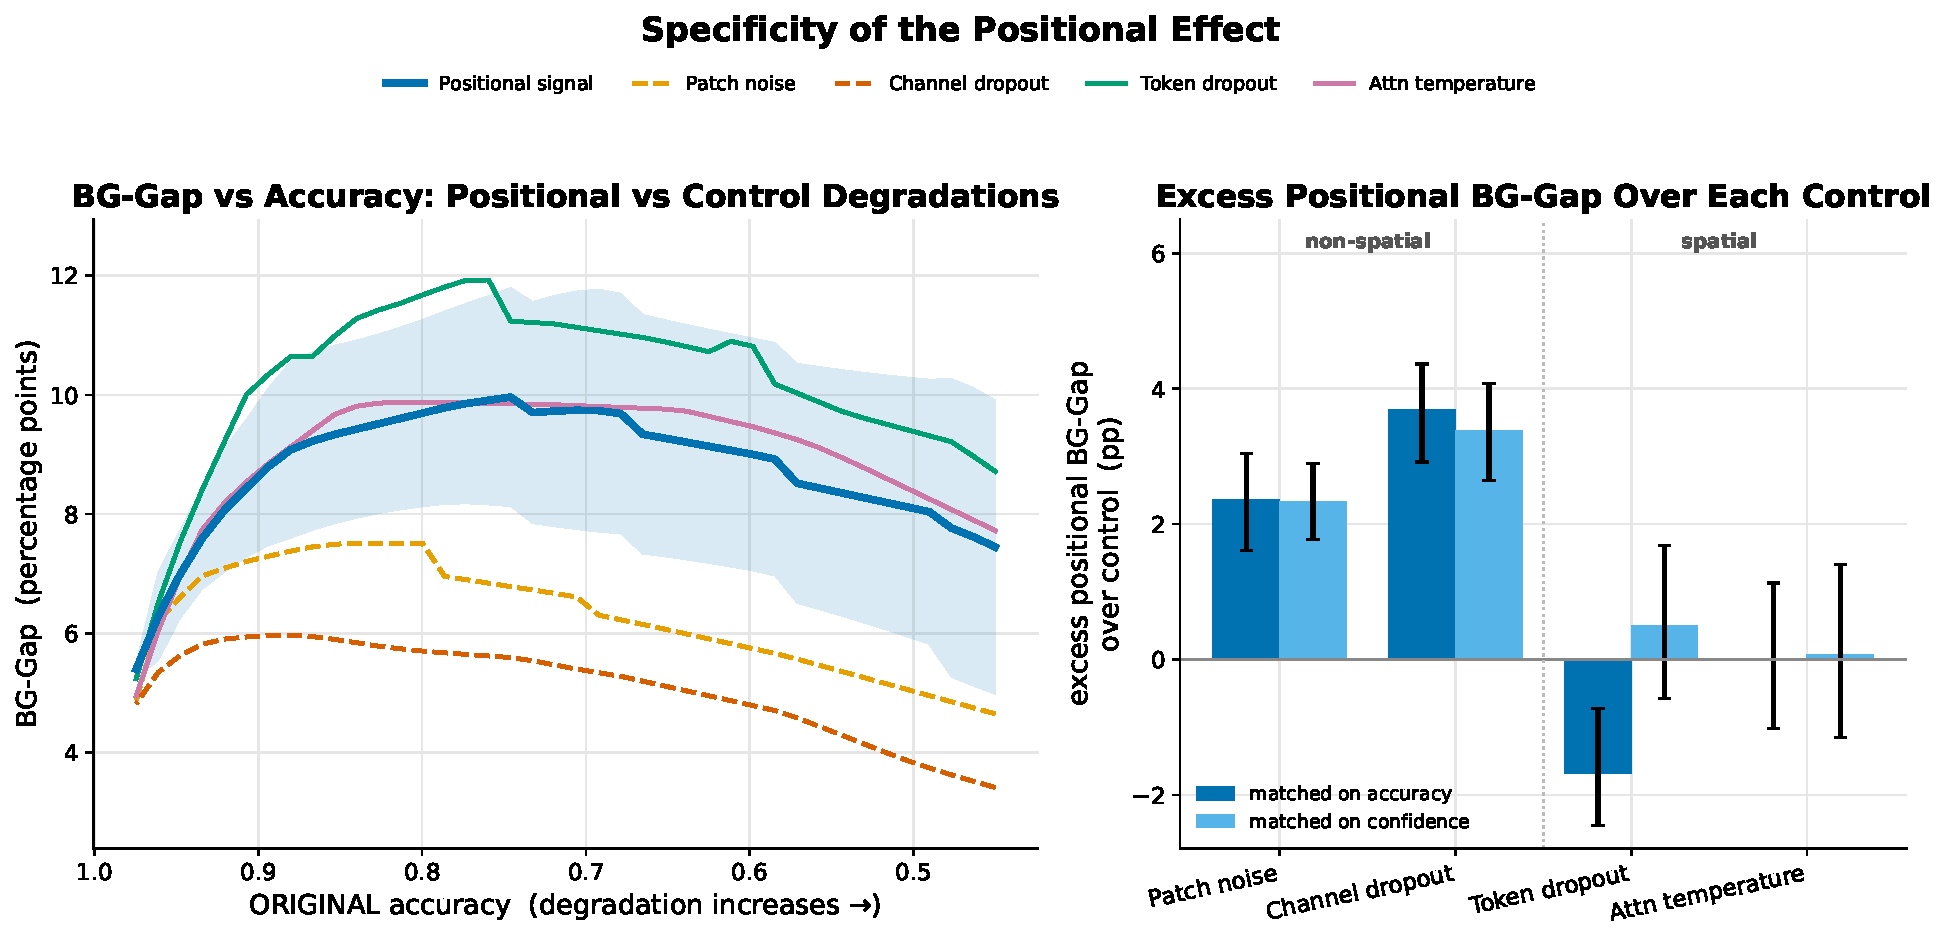
\includegraphics[width=\linewidth]{figures/09_specificity_curve.pdf}
  \caption{\textbf{Position-specific, not generic degradation.} Excess $\mathrm{BG\text{-}Gap}$ of
    positional attenuation over accuracy-matched controls; positive vs.\ non-spatial controls, on par
    with spatial ones.}
  \label{fig:specificity}
\end{figure}

\begin{table}[t]
  \centering\small
  \setlength{\tabcolsep}{3.5pt}
  \begin{tabular}{@{}lcc@{}}
    \toprule
    Control (what it degrades) & $\Delta$@acc (pp) & $\Delta$@conf (pp) \\
    \midrule
    Patch-noise (feature fidelity)  & \textbf{+3.77} & \textbf{+4.32} \\
    Attn-temperature (routing)      & +1.25 & +2.76 \\
    Token-dropout (spatial)         & $-0.99$ & +0.86 \\
    \bottomrule
  \end{tabular}
  \caption{Excess $\mathrm{BG\text{-}Gap}$ of positional attenuation over each control at matched
    accuracy / matched confidence (mean over 8 models). Positive $=$ position-specific. \textbf{Bold}
    $=$ largest excess.}
  \label{tab:specificity}
\end{table}

\subsection{Generalization, Robustness, and What Governs the Shortcut}
We then test external validity and what governs the shortcut. On Waterbirds (\cref{fig:general}a), removing positional information widens the spurious gap in $5/5$ encodings under the outlined accuracy guard, with a gap spread of $1.9$\,pp that remains encoding-agnostic. The witnessed phenomena is observed to be governed by foreground object size (\cref{fig:general}b): $\mathrm{BG\text{-}Gap}$ falls from $\sim 10$\,pp for the smallest foregrounds to $\sim 1$\,pp for the largest, identically across encodings. This re-confirms~\cite{xiao2021} and, further, the causal result: it is robust to the specific attenuation (low-pass, frequency-truncation) and concentrates in later layers.

\begin{figure*}[t]
  \centering
  \begin{subfigure}{0.49\linewidth}
    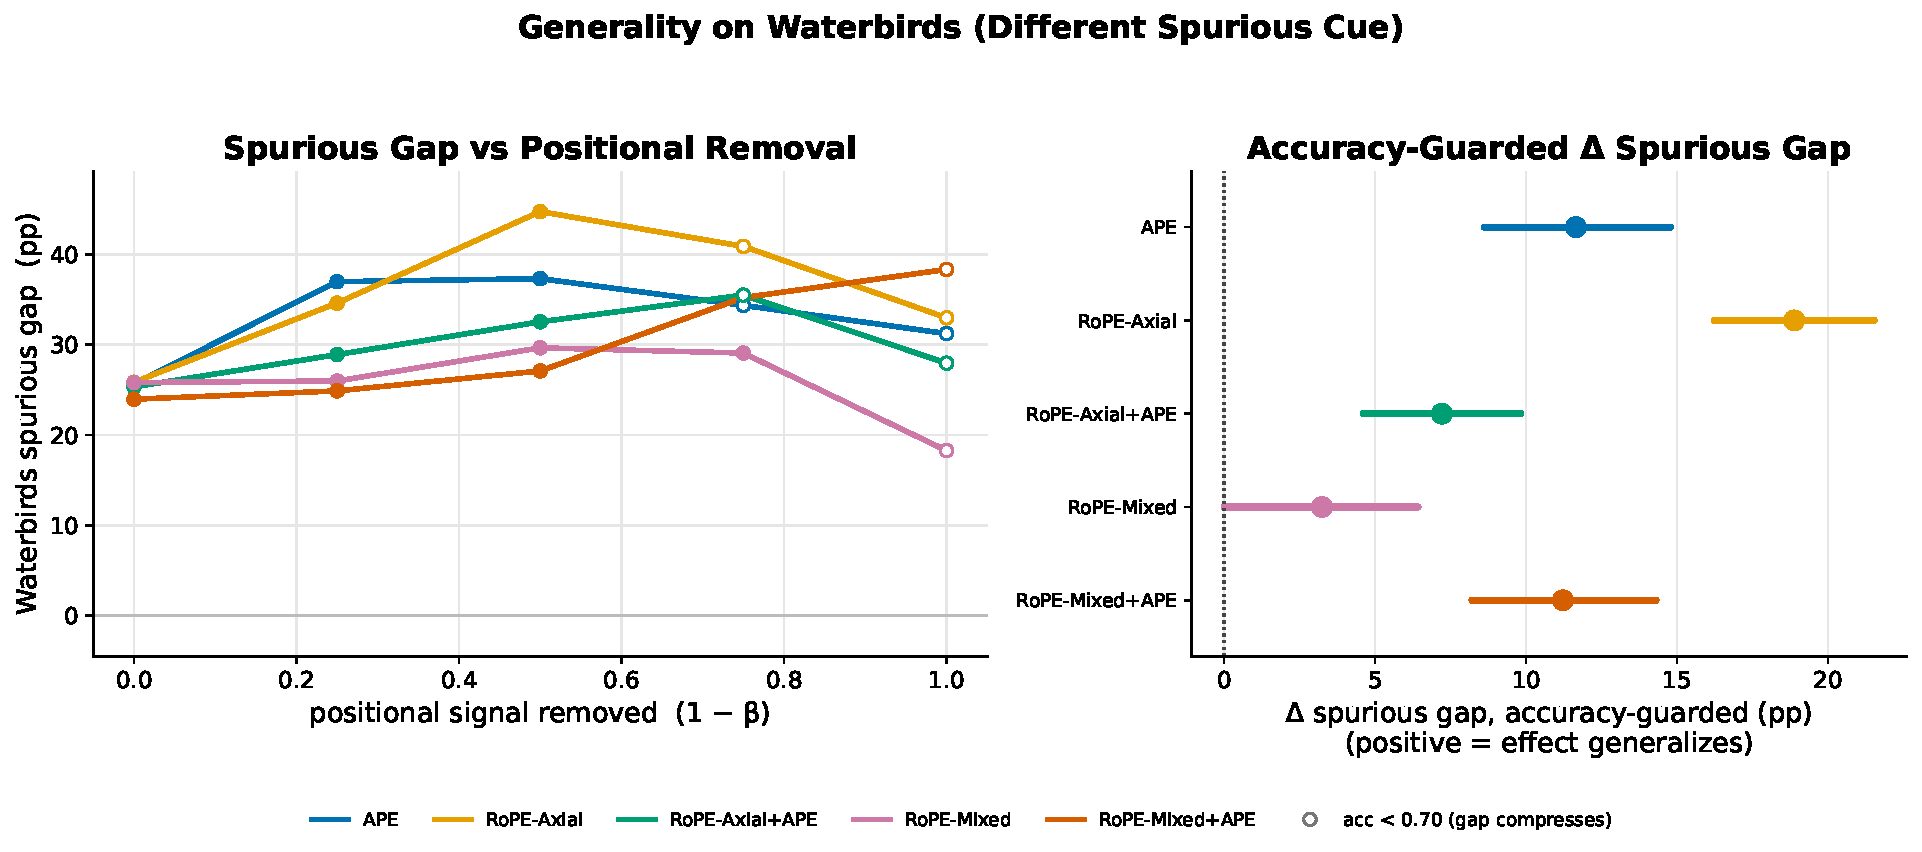
\includegraphics[width=\linewidth]{figures/12_waterbirds_generality.pdf}
    \caption{Waterbirds: 5/5 encodings widen the spurious gap.}\label{fig:general-wb}
  \end{subfigure}\hfill
  \begin{subfigure}{0.49\linewidth}
    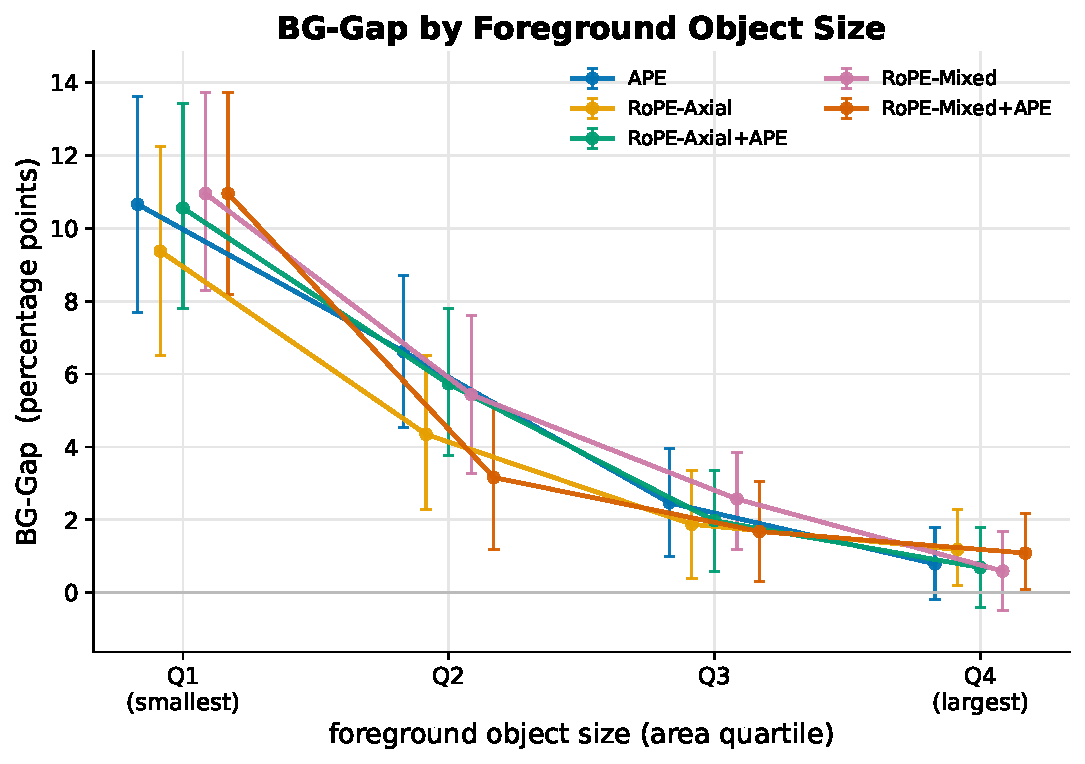
\includegraphics[width=\linewidth]{figures/06_object_size.pdf}
    \caption{Object size governs reliance ($\sim$10\,pp $\to$ $\sim$1\,pp).}\label{fig:general-size}
  \end{subfigure}
  \caption{\textbf{The effect generalizes and is governed by object size.}}
  \label{fig:general}
\end{figure*}

\subsection{Investigating Candidate Mechanisms}
\label{sec:mechanisms}
Finally we ask what carries the observed effect. We investigated four plausible mechanisms and found little evidence that any single channel does (\cref{tab:mech}): while per-image attention entropy can predict background-reliant images (AUC $0.70\,[0.67,0.72]$; $\mathrm{BG\text{-}Gap}$ rising $0.4 \to 11.5$\,pp across entropy quartiles), register/artifact tokens are \emph{anti}-predictive of per-image reliance (AUC $0.35$); a causal attention-temperature sweep is null or reversed; background decodability \emph{falls} rather than rises as the gap grows; and a high-frequency rotary band shows $\approx 0$\,pp excess at matched accuracy. Further on per-image attention entropy, it is likely merely a vehicle for difficulty as it does not transfer to Waterbirds (AUC $\approx 0.54$).

\begin{table*}[t]
  \centering\small
  \begin{tabular}{@{}lll@{}}
    \toprule
    Candidate mechanism & How tested & Result \\
    \midrule
    Artifact/``register'' tokens     & per-image AUC          & 0.35 (anti-predictive) \\
    Attention geometry/routing       & attn-temp sweep & null / reversed \\
    Background decodability          & linear probe vs.\ $\beta$ & falls as gap rises \\
    High-frequency rotary band       & excess @ matched acc.  & $\approx 0$\,pp (deny) \\
    \midrule
    Attention entropy (spread)       & per-image AUC          & 0.70\,[0.67,0.72] \emph{(diagnostic)} \\
    \bottomrule
  \end{tabular}
  \caption{Four candidate mechanisms are unsupported; one correlational diagnostic survives. The effect
    resists single-channel localization.}
  \label{tab:mech}
\end{table*}

%------------------------------------------------------------------------
\section{Discussion}

\subsection{What It Means}
The results support a single qualified conclusion: the functional positional signal causally constrains a Vision Transformer's reliance on the background shortcut. Three observations qualify it. First, the constraint is a property of the positional information, not its encoding---attenuating the used signal raises reliance in every model while the unused copy is inert, and APE, RoPE, and hybrid variants are statistically equivalent. Second, the effect is spatial, exceeding accuracy-matched feature-fidelity controls. Third, this finding is not an artifact of one benchmark, as the results are replicated on Waterbirds and affected by object sizes as prior works would predict.

\subsection{The Frontier: Real but Distributed}
A natural next question is what carries the constraint. We investigated four candidates: artifact tokens, attention geometry, background decodability, and a high frequency rotary band (to RoPE dimensions that encode more minute positional changes), finding little evidence that one of these channels carries the effect. As such, the constraint, empirically, seems to resist single-channel localization, instead having a more distributed effect.

\subsection{Necessity, Not Sufficiency}
Our evidence remains unbalanced. Removing positional signal consistently increases background reliance, but amplifying it does nothing, with every CI for amplification crossing zero and the intact model already sitting near its background-reliance minimum. Therefore, we describe positional information as constraining the shortcut rather than further safeguarding from it.

\subsection{Limitations}
\label{sec:limitations}
There were several limitations. Firstly, we only had one checkpoint per encoding with a single seed per encoding, so between-encoding comparisons carry the theoretical idiosyncrasies of each checkpoint. As our causal claims are within checkpoints to defuse this, some of the adverse effects of this are mitigated, but controlled multi-seed training remains. Next, we only used two benchmarks: ImageNet-9 and Waterbirds, which are two related ``spurious background'' benchmarks, limiting the generality of our results. With regards to signals, the entropy diagnostic is correlational and likely confounded. Ultimately, the mechanism for BG reliance is unresolved.

\subsection{Lessons Learned}
While creating this project, beyond learning more about transformers in general, I learned a significant amount about good experimental design in machine learning. While I was originally frustrated that the nullification of my hypothesis without another clear direction left my findings unsatisfying at best, the project taught me to follow the data over the hypothesis. Along this path, I learned a failed but rigorous attempt at searching for a key finding can be just as insightful as a clean result. Finding clean results, I learned, also comes with its own complications. Compute and tooling limits; in particular, time limits because of the tight frame of this project showed me how I needed to leverage statistics and good experimental design over trying to, for instance, repeatedly retrain vision transformers. This required me to challenge my assumptions---if there is one thing I learned, it is that there is a large difference between something being intuitive and well established.

%------------------------------------------------------------------------
\section{Conclusion}

\subsection{Summary}
In this work, we tested whether positional information causally constrains a Vision Transformer's reliance on the background shortcut. We did this by scaling the positional signal of eight frozen, identically-trained models that use different positional encoding schemes and measuring the changes in background reliance. We found that attenuating this functional signal monotonically increases reliance across all eight checkpoints independently of encoding scheme with, keyly, APE and RoPE being statistically equivalent. This reflects loss of spatial information specifically, generalizing to a second spurious benchmark. Because removal raises reliance while amplification does not, we describe positional information as constraining rather than safeguarding from the background shortcut---it is necessary, but not sufficient.

\subsection{Future Work}
There are several potential directions following this work. Firstly and most apparently, multi-seed training with a positional-robustness objective, such as through positional dropout, would help work towards proving that positional information is sufficient for proving background reliance. Secondly, distributed causal tracing could potentially localize the effect or establish more rigorously that it has no single channel. Third, if the observed constraint can become stronger, it could serve as a cheap, retraining-free adjustment for robustness.

In application, testing whether the principle that a model's sense of place constrains spurious reliance holds for video, medical, satellite, or other large, foundational models could help work towards forming a safeguard against these behaviors. Through these sensitive fields, the measured benefit of limiting background reliance could be evidenced.

Our analysis uses only released checkpoints, adding no generative capability and instead primarily being diagnostic.


%%%%%%%%% REFERENCES
{\small
\bibliographystyle{ieee_fullname}
\bibliography{egbib}
}

\end{document}
